% !Mode:: "TeX:UTF-8"
\chapter{SNO+实验}

SNO+(Sudbury Neutrino Observatory+)实验是一个位于加拿大安大略省的SNOLAB
(Sudbury Neutrino Observatory Laboratory,萨德伯里实验室)的实验。该实验的低背景,
高分辨率,很适合开展多方面的中微子研究,例如反应堆中微子,太阳中微子,
超新星中微子等。SNO+实验的主要科学目标是探测极为罕见的无中微子双贝塔衰变
(0$\nu\beta\beta$)。为实现这一雄心勃勃的目标,
SNO+分阶段在一个直径12米的丙烯酸容器中先后装载了纯水(2017-2019年),780吨液体闪烁体
(2019-2024年),
并计划向其中加入约1.3吨的同位素$^{130}\mathrm{Te}$(碲-130)(预计2025年开始)
\cite{andringa2016current}。

这一章主要介绍SNO+实验,\ref{goal}节简要介绍了SNO+实验的物理目标,
\ref{facility}节简要介绍了SNO+实验的实验装置,
\ref{background}节简要介绍了SNO+实验中的部分背景事件。

\section{物理目标}\label{goal}

SNO+实验的主要科学目标是使用${}^{130}$Te探测一种极为罕见的物理现象——无中微子双贝塔衰变
(0$\nu\beta\beta$)。这一现象在\ref{sec:double_beta_decay}节中已经介绍过了。
如果观测到这一现象,将对中微子物理和基本粒子理论产生深远的影响。目前根据COURE实验
的结果,对于${}^{130}$Te的2$\nu\beta\beta$衰变的半衰期为:\cite{PhysRevLett.126.171801}
\begin{equation}
    T_{1/2}^{2\nu} = 7.71^{+0.08}_{-0.06}(stat.)^{+0.12}_{-0.15}(syst.)\times10^{20}~\mathrm{yr}
    \label{eq:2vbb}
\end{equation}

End point能量为:\cite{PhysRevC.80.025501}

\begin{equation}
    Q_{\beta\beta} = 2527.518 \pm 0.013~\mathrm{keV}
    \label{eq:Qbb}
\end{equation}

${}^{130}$Te相对其他同位素具有很多优势,包括其较高的自然丰度(34.1\%),
以及相对更便宜的价格。这使得我们可以在不进行富集的情况下大批量地投入使用。
同时,${}^{130}$Te的2$\nu\beta\beta$衰变的半衰期也相对较长,这使得
不可减少的2$\nu\beta\beta$背景事件被压低了。

除了0$\nu\beta\beta$之外,SNO+实验还可以用于其他的中微子研究,
例如低能量的太阳中微子,地球中微子,反应堆中微子等。SNO+探测器
同时还可以作为一个超新星中微子监测器。

\section{SNO+实验装置}\label{facility}

SNO+实验的选址位于地下2.1km的SNOLAB。等效水深约为6010m,可以有效地屏蔽宇宙射线。
SNO+复用了SNO实验的探测器,并进行了升级。SNO+探测器的主要结构
由一个厚度为55 mm,直径为12 m的球形透明的
AV( acrylic vessel,丙烯酸容器 )组成,用来装载780吨液体闪烁体,包括LAB(linear alkyl benzene,线性烷基苯)
,PPO(2,5-diphenyloxazole,2,5-二苯基恶唑)以及bis-MSB(1,4-bis(2-methylstyryl)-benzene,1,4-双(2-甲基苯乙烯基)苯)。
AV由直径17.8 m的PSUP( geodesic steel structure,测地钢结构 )环绕,
PSUP内设有9362个带有低活性玻璃和聚光器的内向型PMT( photomultiplier tubes,光电倍增管 )。
91个没有聚光器的PMT也被安装在朝向探测器外的地方,
以探测来自μ子和PSUP外部区域的其他光源的光。
AV和PMT之间以及包含探测器的其余腔体的体积由7000吨超纯水( UPW )填充。
这个外部水量为来自PSUP和空腔墙的AV提供了数米的屏蔽,
这两个空腔墙都是外部辐射的来源。如图\ref{fig:sno+facility}所示。

\begin{figure}[htbp]
    \centering
    \begin{minipage}
        [htbp]{0.45\textwidth}
        \centering
        % Adjust the width (e.g., to 0.8\textwidth) to reduce height while keeping aspect ratio
        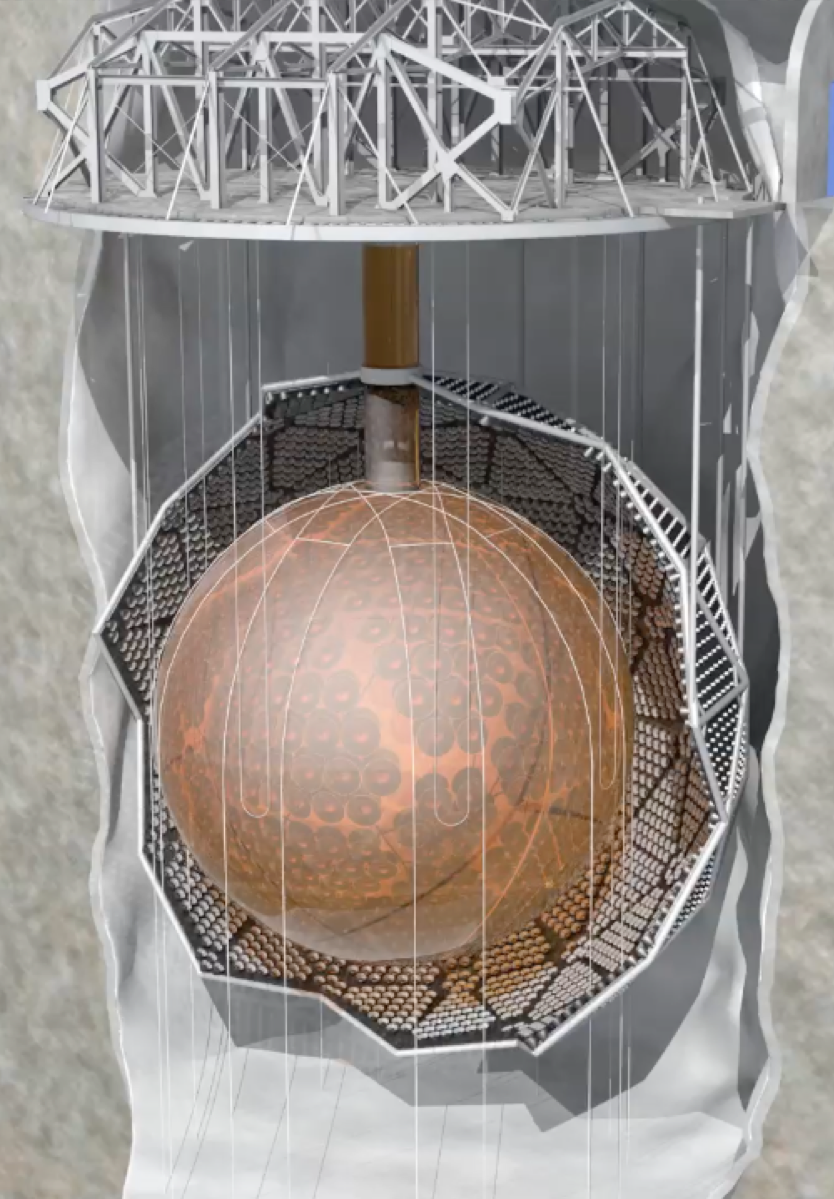
\includegraphics[width=0.85\textwidth]{figures/cavity.png}
    \end{minipage}
    \hfill % or \hspace{\fill}
    \begin{minipage}[htbp]{0.45\textwidth}
        \centering
        % Adjust the width (e.g., to 0.8\textwidth) to reduce height while keeping aspect ratio
        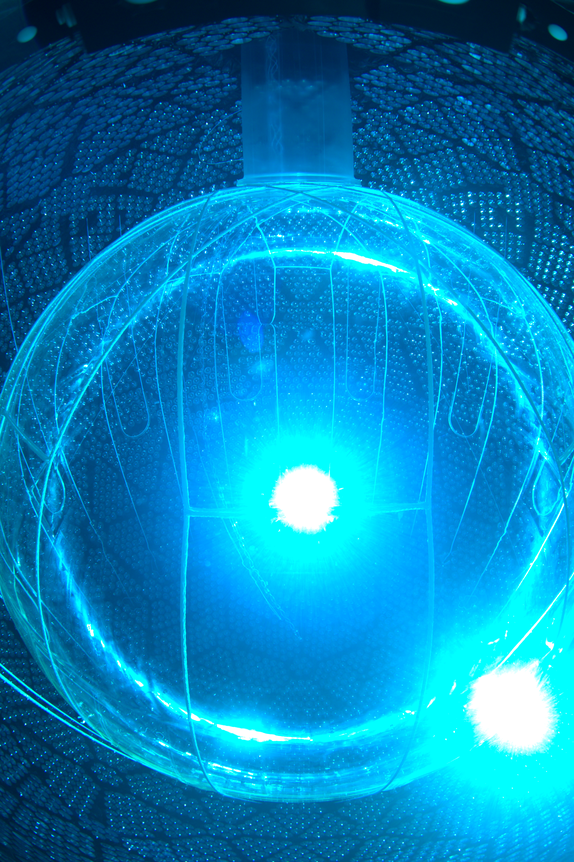
\includegraphics[width=0.85\textwidth]{figures/photograph.png}
    \end{minipage}
    \caption{左边是SNO+实验装置的示意图\cite{andringa2016current},右边是SNO+实验装载纯水时内部的照片\cite{andringa2016current}}
    \label{fig:sno+facility}
\end{figure}

\section{SNO+实验中的背景事件}\label{background}

如果我们要分辨出0$\nu\beta\beta$的微弱信号,
那么准确的背景分析至关重要。
从图\ref{fig:0vbb_2vbb}中,我们可以看出,最终我们要探测的是后面
0$\nu\beta\beta$的峰,也即0$\nu\beta\beta\quad{}^{130}$Te的$Q$值。
\begin{figure}[htbp]
    \centering
    \begin{minipage}[htbp]{0.45\textwidth}
        \centering
        % Adjust the width (e.g., to 0.8\textwidth) to reduce height while keeping aspect ratio
        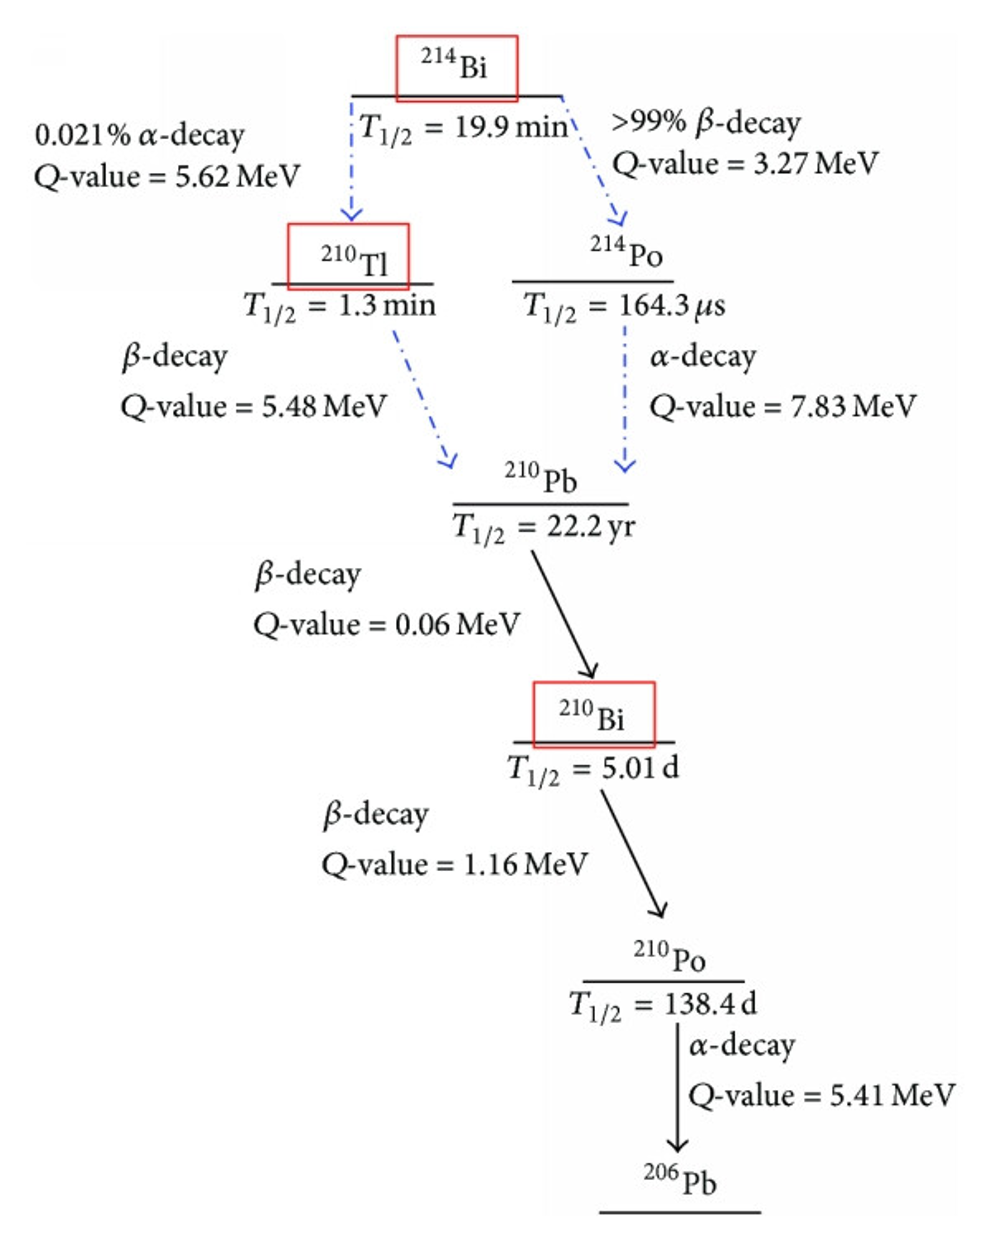
\includegraphics[width=0.85\textwidth]{figures/BiPo214.png}
    \end{minipage}
    \hfill % or \hspace{\fill}
    \begin{minipage}[htbp]{0.45\textwidth}
        \centering
        % Adjust the width (e.g., to 0.8\textwidth) to reduce height while keeping aspect ratio
        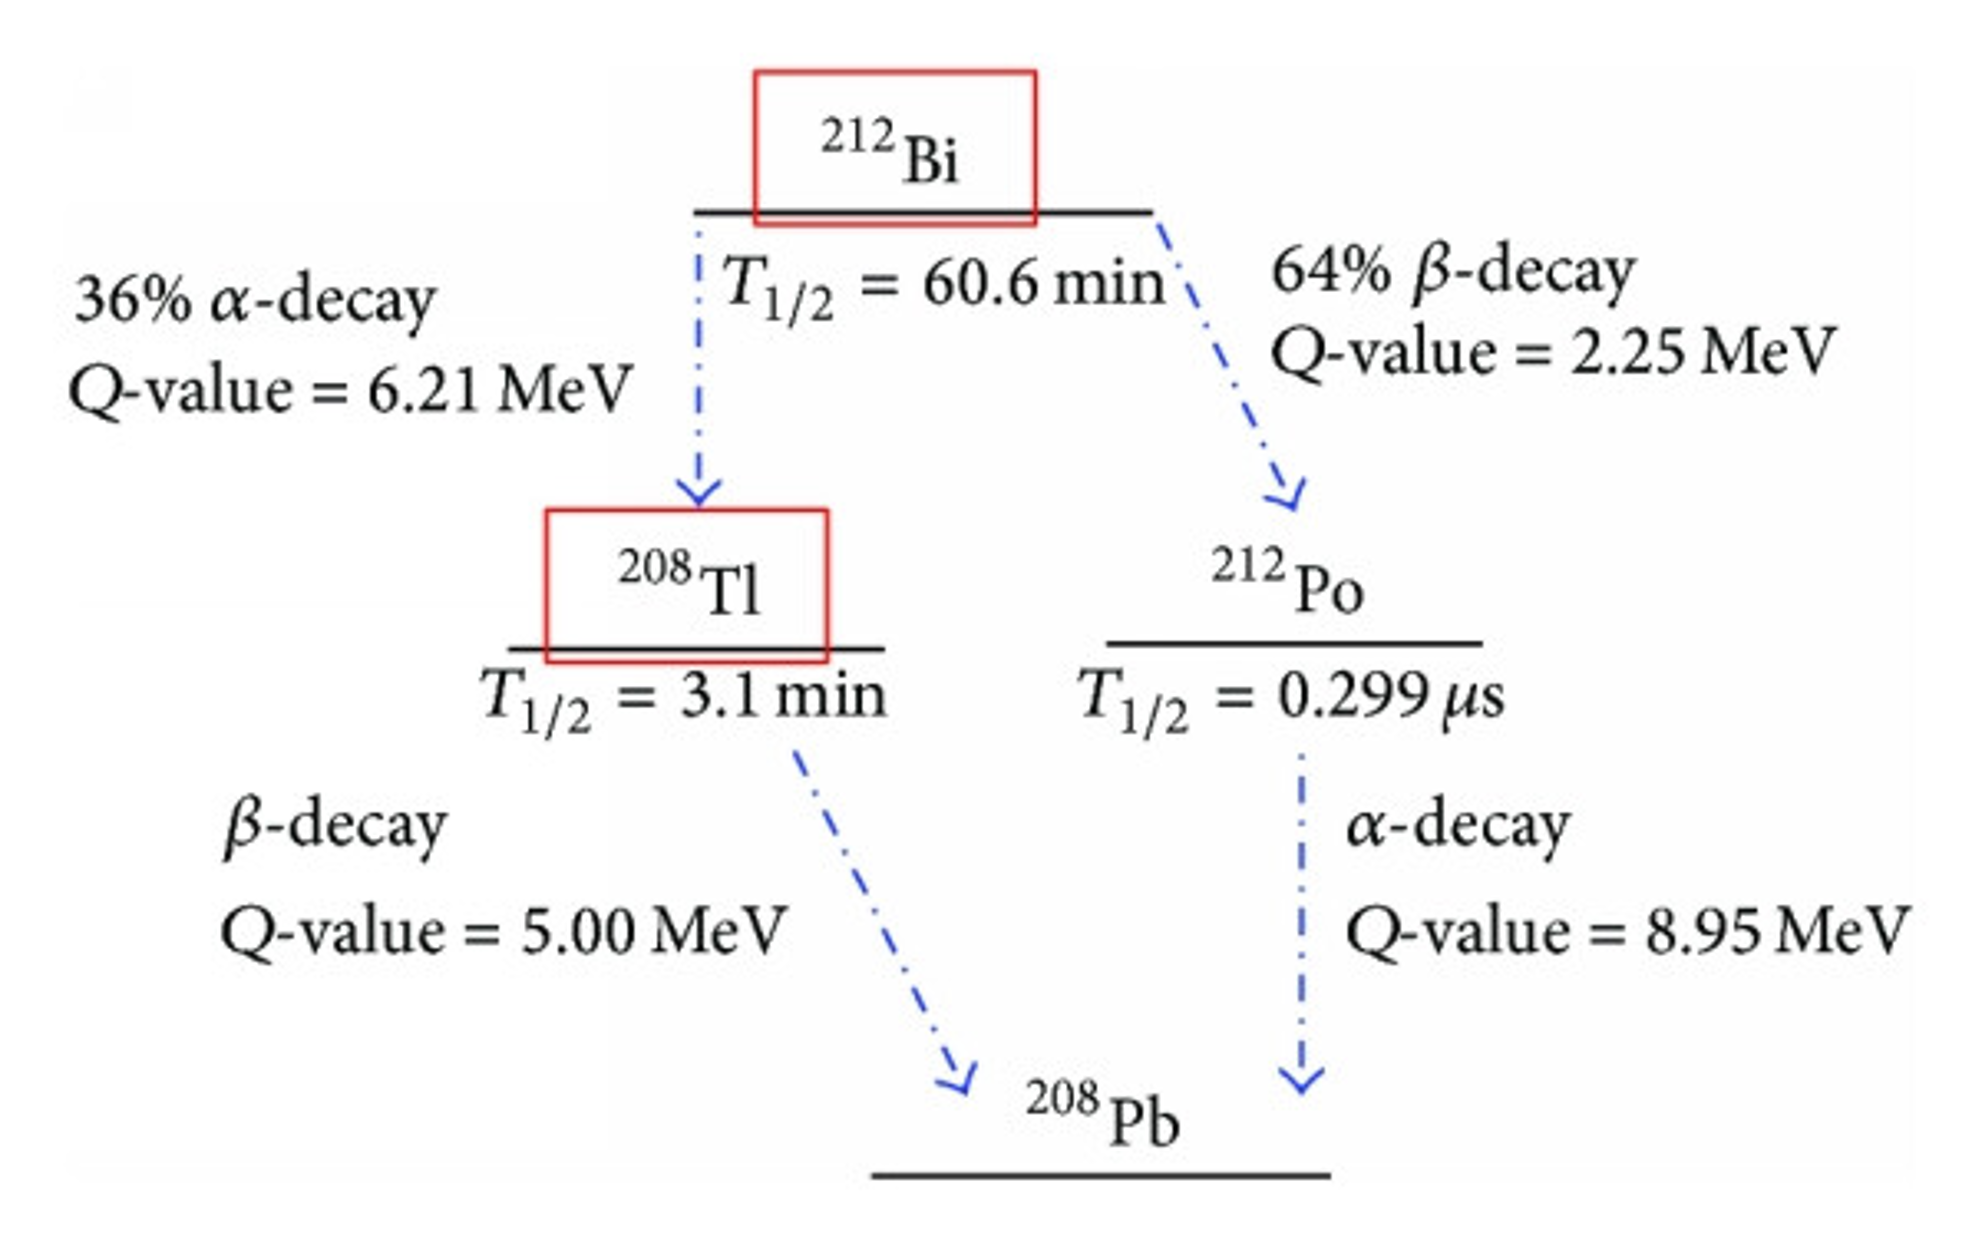
\includegraphics[width=0.85\textwidth]{figures/BiPo212.png}
    \end{minipage}
    \caption{SNO+实验中${}^{214}$Bi-${}^{214}$Po和${}^{212}$Bi-${}^{212}$Po衰变的$Q$值\cite{andringa2016current}}
    \label{fig:bipo212/214}
\end{figure}

对于这一同位素,
从表\ref{tab:bb}中我们知道,其$Q$值约为2.5MeV。故SNO+中的背景分析
需重点关注其($-0.5\sigma,1.5\sigma$)内,即大约2.47-2.69MeV的事件。重点关注的背景事件有
${}^{214}$Bi-${}^{214}$Po,${}^{212}$Bi-${}^{212}$Po,${}^{8}$B太阳中微子等。


从NNDC(National Nuclear Data Center,国家核数据中心),
以及图\ref{fig:bipo212/214}中
${}^{212}$Bi-${}^{212}$Po和${}^{214}$Bi-${}^{214}$Po衰变的$Q$值
,我们可以看到,图中$Q$值并不位于2.5MeV附近,然而由于量子淬灭效应,
使得实际在SNO+探测器中探测到的$Q$值会偏低。\cite{bvkrosigk2015}
这样,这个衰变($\beta-\alpha$衰变中的$\alpha$衰变)的$Q$值会落在这一范围内。

\begin{figure}[htbp]
    \centering
    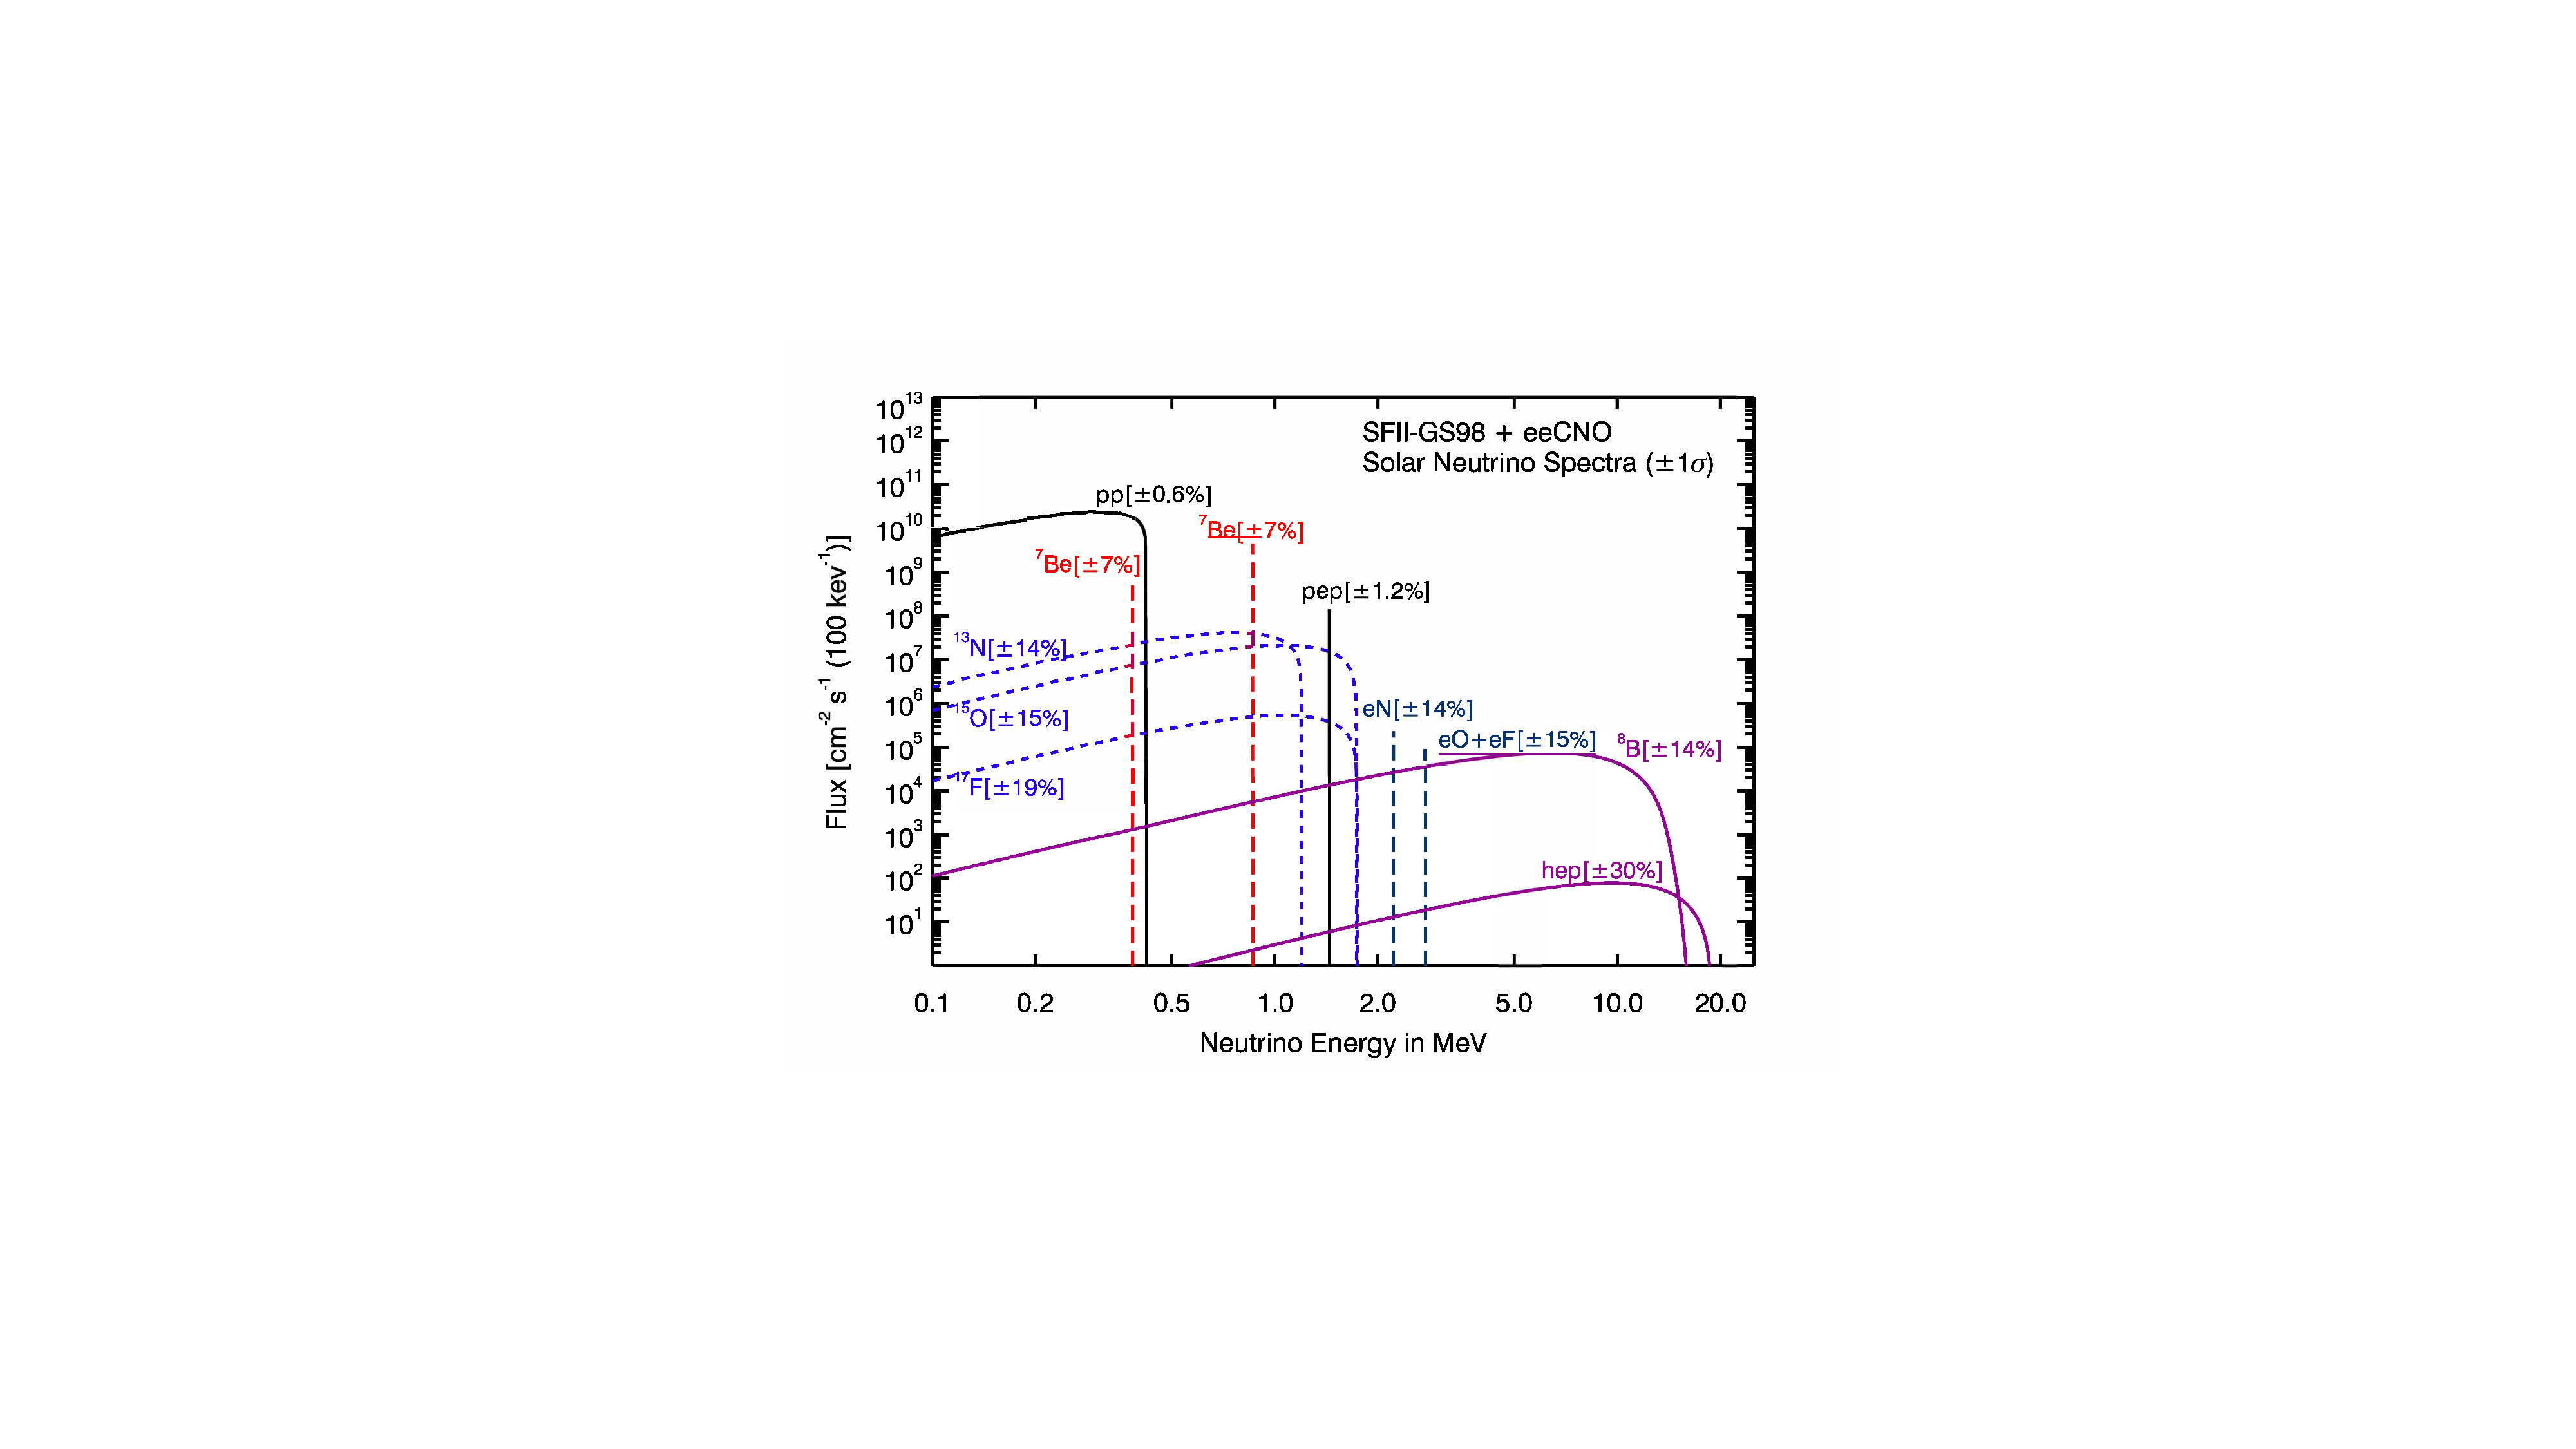
\includegraphics[width=0.6\textwidth]{figures/solarnuspec.pdf}
    \caption{太阳中微子能谱\cite{ParticleDataGroup:2024cfk}}
    \label{fig:solarnu}
\end{figure}


而对于${}^{8}$B太阳中微子,我们从图\ref{fig:solarnu}中可以看到,
根据标准太阳模型,太阳光谱中${}^{8}$B中微子能谱的分布覆盖了0.1-15MeV的范围,
当然也包括了2.5MeV附近的范围。我们可以看到,${}^{8}$B中微子这一能量
附近的流强约为10${}^4$cm$^{-2}$s$^{-1}$(100kev${}^{-1}$)量级。

在所有${}^8$B太阳中微子的衰变道中,这一能量附近的${}^8$B中微子的衰变道中,
只有弹性散射(ES,elastic scattering)会发生,即
\begin{equation}
    \nu_e + e^- \rightarrow \nu_e + e^-
\end{equation}
故探测到的是一个单信号(即电子的信号)。因此
${}^8$B太阳中微子也是一个重要的背景事件。

\section{小结}\label{summary}

本章首先介绍了SNO+实验的基本情况,包括其地理位置、发展阶段以及主要科学目标——探测${}^{130}$Te的无中微子双贝塔衰变。
接着,详细阐述了SNO+的物理目标,不仅包括核心的0$\nu\beta\beta$探测,还涵盖了太阳中微子、地球中微子、反应堆中微子以及超新星中微子等其他研究方向,并解释了选择${}^{130}$Te作为目标同位素的优势。
随后,本章描述了SNO+实验的装置,包括其深地实验室的位置、探测器的主要组成部分(如丙烯酸容器、液体闪烁体、光电倍增管阵列和外部超纯水屏蔽层)。
最后,讨论了SNO+实验中对0$\nu\beta\beta$探测构成挑战的主要背景事件,重点分析了${}^{214}$Bi-${}^{214}$Po、${}^{212}$Bi-${}^{212}$Po衰变链以及${}^{8}$B太阳中微子弹性散射事件,这些事件的能量可能落在感兴趣的区域内,需要精确识别和扣除。
这些背景事件在下一章都会成为我们在机器学习中需要用到的数据集。